Nous représenterons ici de manière schématique les fonctionnalités de l’outil.

\bigbreak

\subsection{Diagramme de cas d’utilisation}

\begin{figure}[!h]
    \center
    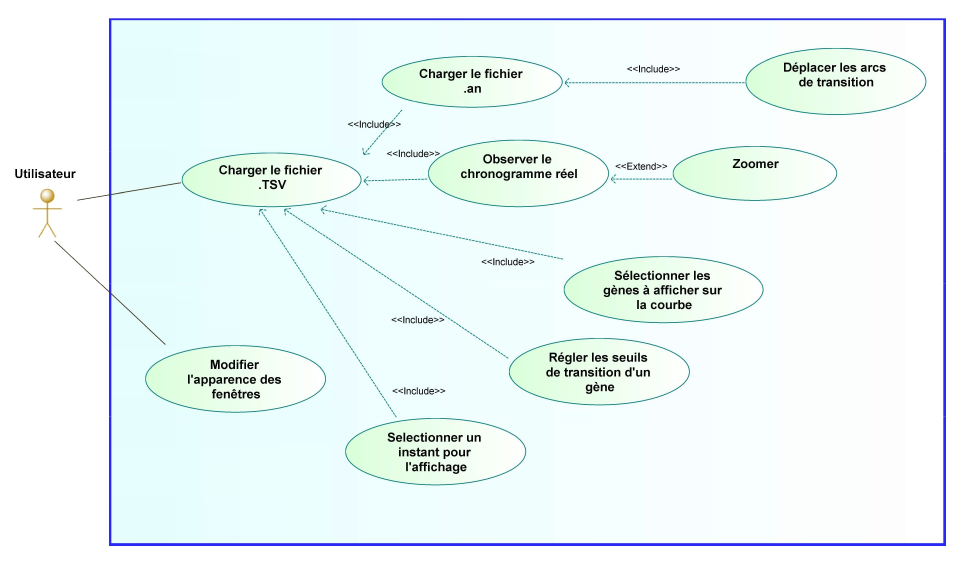
\includegraphics[scale = .65]{images/utilisation.png}
   \caption{Diagramme d'utilisation}
 \end{figure}

\bigbreak

\subsection{Diagrammes de séquence}
\bigbreak
Deux composantes de l’application, les fenêtres et le RangeSlider, peuvent fonctionner indépendamment de l’outil. Nous les présenterons donc de manière séparée.
\bigbreak
\newpage
\subsubsection{Fonctionnement des fenêtres}
\bigbreak
Les deux fenêtres ont un mécanisme similaire représenté par le diagramme suivant :
\begin{figure}[!h]
  \bigbreak
  \centering
  \includegraphics[scale = .34]{images/sequence_fenetres.png}
\end{figure}

Leur comportement est proche de celui des fenêtres que nous utilisons au quotidien dans les différents systèmes d’exploitation, à savoir la possibilité de les réduire, de les déplacer et de les redimensionner.

\bigbreak
\subsubsection{Fonctionnement du RangeSlider}
\bigbreak
Afin de faciliter le positionnement des différents curseurs dans le graphe, nous avons implémenté un composant adapté à nos besoins.

\begin{figure}[!h]
  \bigbreak
  \centering
  \includegraphics[scale = .4]{images/sequence_slider.png}
\end{figure}

\bigbreak

Ce composant est très intuitif à utiliser. Il sera présenté plus en détails dans la partie 4.4. On peut observer que la grande majorité des traitements sont effectués en interne par l’objet. En effet, il a été codé de manière non spécifique au projet afin de pouvoir être réutilisé facilement à plusieurs endroits, avec toutefois quelques légères variations inhérentes aux besoins de l’application.

\bigbreak

\subsubsection{Fonctionnement global de ViMaSTBio}

Ce diagramme résume une bonne partie des fonctionnalités disponibles dans l’application. Le déplacement des flèches de transition des automates n’est pas représenté par souci de clarté, car leur mécanisme est presque identique à celui du déplacement des fenêtres, à la différence près qu’à chaque mouvement une courbe d’interpolation (une courbe de Bézier) est calculée et dessinée.

\begin{figure}[!h]
  \bigbreak
  \centering
  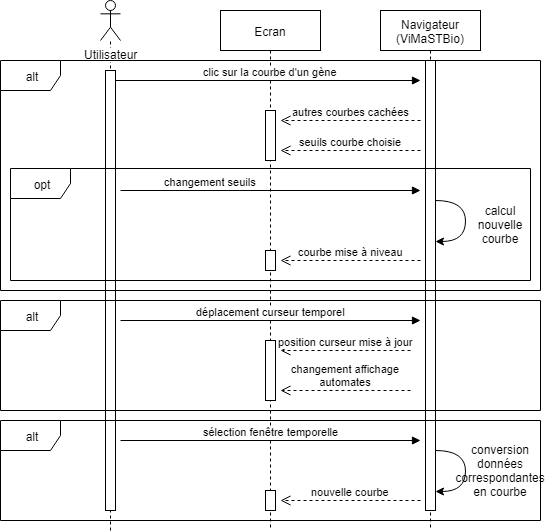
\includegraphics[scale = .4]{images/sequence.png}
\end{figure}
\bigbreak
La grande quantité d’informations circulant entre les blocs est liée à la nature de l’outil qui demande précisément de mettre en relation ces données. Le regroupement de variables globales est ici essentiel à cause du fonctionnement de Javascript (cf la présentation de la page html), et présente le double avantage de simplifier les échanges.
